\section{Программная реализация алгоритма и визуализация}

Для автоматизации расчетов и генерации данных, частично представленных в таблице~\ref{tab:metrics}, использовался программный модуль, разработанный на языке \texttt{C++}. Ниже представлен листинг~\ref{code:cpp_script}, загруженный напрямую из файла проекта с помощью возможностей пакета \texttt{minted}.

\inputminted[label=script.cpp]{cpp}{script.cpp}
\label{code:cpp_script}

В коде функция \mintinline{cpp}{calculateFactorial(n)} использует классический рекурсивный подход. Обратите внимание, что имя переменной \texttt{n} внутри исходного кода семантически совпадает с обозначением в формуле~\eqref{eq:sum}. Дополнительные материалы по реализации похожих курсов можно найти на ресурсе~\cite{fkn}.

\subsection{Иллюстрация результатов работы}

Для визуализации математических объектов обратимся к рисункам. На рисунке~\ref{fig:first_graph} схематично изображён график распределения плотности вероятностей, а на рисунке~\ref{fig:second_graph} показана общая структурная схема разработанного программного обеспечения.

\begin{figure}[htbp]
    \centering
    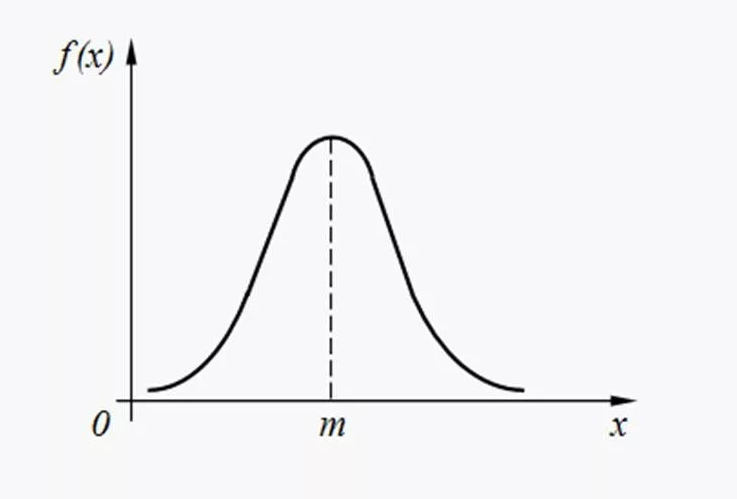
\includegraphics[width=0.5\textwidth]{image1.png}
    \caption{График распределения функции}
    \label{fig:first_graph}
\end{figure}

\begin{figure}[htbp]
    \centering
    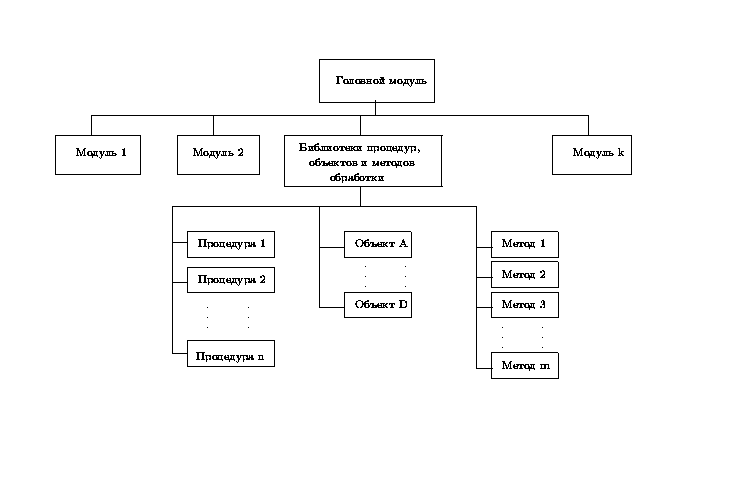
\includegraphics[width=0.5\textwidth]{image2.png}
    \caption{Структурная схема программного модуля}
    \label{fig:second_graph}
\end{figure}

Использование Docker-контейнеризации~\cite{docker-docs} позволяет изолировать выполнение данного программного кода.